\documentclass[sunil1]{sunil} %See documentation for other class options
%\documentclass[sunil1,ChapterTOCs]{sunil} %See documentation for other class options
\usepackage{fixltx2e,fix-cm}
\usepackage{amssymb}
\usepackage{amsmath}
\usepackage{graphicx}
\usepackage{subfigure}
\usepackage{makeidx}
\usepackage{multicol}
\usepackage{paralist}
\newcommand{\comment}[1]{\textcolor{red}{{\bf#1}}}


\frenchspacing
\tolerance=5000

\makeindex

%\bibpunct{[}{]}{;}{n}{,}{,} % square brackets
% "Greater/Less than or of order" symbols
\def \la {\mathrel{\vcenter
     {\hbox{$<$}\nointerlineskip\hbox{$\sim$}}}}
\def \ga {\mathrel{\vcenter
     {\hbox{$>$}\nointerlineskip\hbox{$\sim$}}}}

% \textwidth 6.1in
% \textheight 8.25in
% \oddsidemargin 0.24in
%\evensidemargin -0.5in
%\topmargin -0.25in

\begin{document}

\title{Software Process for Multicomponent Multiphysics
  Codes}

\tableofcontents
%\include{foreword}
%\include{preface}
%\listoffigures
%\listoftables
%\include{contributor}
%\include{symbollist}

\mainmatter

\chapterauthor{Anshu Dubey}{ANL}
\chapterauthor{Katherine Riley}{ANL}
\chapterauthor{Katie Antypas}{LBL}




% \begin{abstract}
% Multiphysics multicomponent scientific codes have increasingly been 
% adopting software processes derived from outside the scientific
% domain. The driving force behind adoption is usually the realization
% that without using software engineering practices, the development,
% verification and maintenance of code becomes intractable. However,
% many software best practices need modification and/or customization.
% Sometimes the inherent physics of scientific applications require
% different software methodologies, while other times a premium is
% placed on performance rather than architecture.  Still others are more
% sociological and due to the type of institutions that are the typical
% homes for such codes. The challenges for scientific applications range
% from their architecture to the process for their maintenance and
% growth. For example, sometimes modularity and encapsulation principles
% are challenged by the need to tightly couple physics solvers to data
% structures.  Scientific codes are designed to explore phenomena that
% are not very well understood, so their verification strategies have to
% be customized. % The components of scientific codes must also consider
% % accuracy and stability, and interoperability between components must not
% % violate physical constraints. These constraints are particularly challenging for
% % numerical software because a wrong answer may not be detected to be wrong
% % because of the exploratory nature of the problems being addressed.  Finally, as
% % the research in the field evolves, codes may have to undergo radical
% % changes in base algorithms to include the newly acquired knowledge. And
% % the metrics of success are harder to define. 
% The institutional challenges in developing and maintaining scientific codes arise because the 
% research institutions in which they are developed often have an unreliable
% funding model and a transient developer population of graduate
% students. 
% % There are
% % rarely enough resources  to have any redundancy in expertise which makes
% % procedures like code review difficult. 
% Intellectual ownership, code 
% distribution, attribution of credit and contribution policies can all
% become thorny issues because there is often a lack of communication
% and sometimes even distrust among the stakeholders. 
% % Documentation
% % takes on a different kind of urgency because of transient expertise,
% % and yet it is notoriously difficult to persuade the 
% % developers in the field to spend their limited time providing
% % exhaustive documentation. 
% We elaborate on the above challenges and
% how they were addressed in FLASH, a code that has been extremely
% successful as a community code for several research communities. We
% outline specific solutions used by FLASH, and discuss their possible
% generalizations that are usable by other similar software 
% efforts. In particular, we address the issues related to software
% architecture and modularization, design of a testing regime,
% unique documentation needs and challenges, use of versioning system 
% for managing projects, and the tension between intellectual property
% management and open science. 
% \end{abstract}

\chapter{Software Process for Multiphysics Multicomponent Codes}
\section {Introduction} 
The computational science and engineering (CSE) communities have a mixed record
of using software engineering and adopting good software
practices. Majority of codes adopt software practices when the size
and composition of the code makes it impossible to make progress
without them. In rarer instances code projects start with an awareness
of the importance of software process and build it into the DNA of the
code. As more codes have crossed the threshold of being manageable
without software engineering they have increasingly been 
adopting software processes derived from outside the scientific
domain. The driving force behind adoption is usually the realization
that without using software engineering practices, the development,
verification and maintenance of code becomes intractable. However,
many software best practices are not well-suited for CSE codes without
modification and/or customization. Sometimes the inherent physics of
scientific applications require different software methodologies,
while other times a premium is placed on performance rather than
code architecture.  Still others are more sociological and due to the
type of institutions that are the typical homes for such codes. The
challenges for scientific applications range from their architecture
to the process for their maintenance and growth. 
% For example,
% sometimes modularity and encapsulation principles are challenged by
% the need to tightly couple physics solvers to data structures.
% Scientific codes are designed to explore phenomena that are not very
% well understood, so their verification strategies have  to

\section{Lifecycle}
\label{sec:lifecycle} 
Scientific software is designed to model some phenomena in the
physical world. The phenomena may be at microscopic level, for example
protein folding, or at extremely large scales, for example galaxy cluster
mergers.  In some applications multiple scales are modeled.  (The term 'physical' used here includes chemical and
biological systems since physical processes are underlying building
blocks for those systems too.) The physical characteristics of the systems being modeled are
translated into mathematical models that are said to describe the
essential features of the behavior of the system being
studied. These equations are then discretized, and numerical algorithms
are used to solve them. In general, there are many more degrees of
freedom in the development and lifecycle of scientific software
that are not encountered elsewhere. (KA NOTE: Do we have any thing to support this claim?  If not I would just delete the sentence as it doesn't help our argument.)

\subsection{Development Cycle}
\label{sec:dev-cycle}
For scientific simulations, modeling begins with equations that describe the
general class of behavior to be studied, for example the Navier-Stokes
equations describe the flow of compressible and incompressible
fluids, and Van-der-vaal equations describe force interactions among
molecules in a material. There may be more than one set of equations
if there are behaviors that are not adequately captured by one set.
In translating the model from mathematical representation to
computational representation two processes go on simultaneously,
discretization and approximation. One can argue that discretization is,
by definition, an approximation because it is in effect sampling
continuous behavior where information is lost between sampling
intervals. This loss manifests itself as error terms in the discretized
equations, but error terms are not the only
approximations. Depending upon the level of understanding of specific
sub-phenomena, and available compute resources, scientists also 
use their judgement to make other approximations. Sometimes, to focus on a
particular behavior, a term in an equation may be simplified or may be even completely
dropped. At other times some physical details may be dropped
from the model because they are not understood well enough by the
scientists.  Or the model itself may be an approximation.  

The next stage in developing the code is finding the appropriate
numerical methods for each of the models. Sometimes good methods exists that
can be used ''as-is''.  Other times, they may need to be customized, or new
methods may need to be developed. There may need to be validation of
the method's applicability to the model if the method is new or
significantly modified. Unless an implementation of the method is
readily available as a third party software (stand-alone or in a
library), it has to be implemented and verified. It is at this stage
that the development of a CSE code begins to resemble that of general
software. The numerical algorithms are specified, the semantics are
understood, and they need to be translated into executable
code. Figure \ref{Fig:dev-cycle} gives an example of the development
cycle of a multiphysics application modeled using partial differential
equations. 

\begin{figure}[!t]
\centering
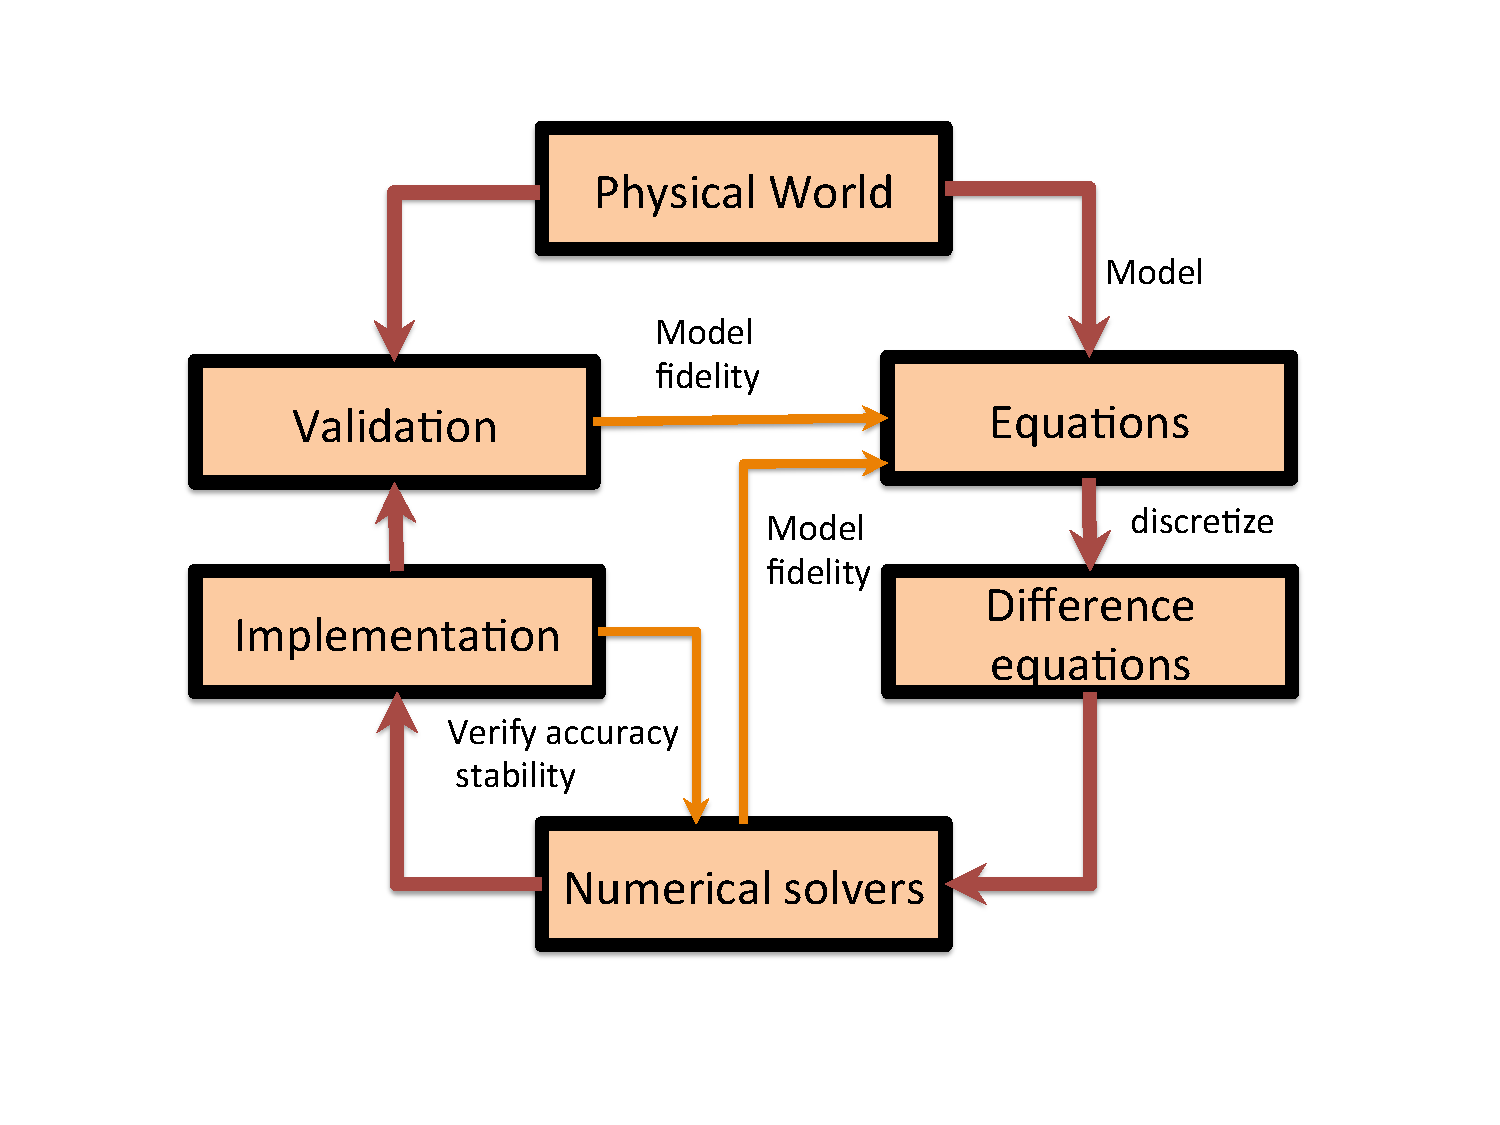
\includegraphics[ width=4.0in]{CSE-design}
\vskip -0.25in
\caption{Development cycle of modeling with partial differential equations}
\label{Fig:dev-cycle}
\end{figure}



\subsection{Verification and Validation}
\label{sec:vandv}
There are many stages in the development cycle of scientific software 
where errors can be introduced. Classes of these errors are mostly
orthogonal to one another, a good verification and validation
methodology will reflect and exploit that.  (KA NOTE: I don't know what the last sentence means...  can you expand a bit?  It pretty vague.)
The terms verification and 
validation are often used interchangeably, but to some communities have specific definitions.  
In one narrow definition, validation, ensures that the
mathematical model correctly defines the physical phenomena, while
verification makes sure that the implementation of the model is
correct. In other words, a model is validated against observations or
experiments from the physical world, whereas a model is verified by other forms of testing.   Other definitions give broader scope to
validation. For example, validation of a numerical
method may be constructed through code-to-code comparisons, and its
order can be validated through convergence studies. Similarly, the
implementation of a solver can be validated against an analytically
obtained solution for some model if the same solver can be
applied and the analytical solution is also known, though this is not
always possible.  Irrespective of  specific definitions, what is true is that
correctness must be assured at all the stages from model to
implementation.  

There are many degrees of freedom in the process of deriving a
model as discussed in the previous section, therefore, the validation of the
model must be carefully calibrated by scientific experts. Similarly,
verification of a numerical method requires applied math expertise
because the method needs verification of its stability, accuracy and
order of convergence, in addition to correctness. Numerical methods
have their own error analysis because of approximations and many of
these methods are themselves objects of ongoing research, so their
implementation may need modifications from time to time. Whenever
this happens, the entire gamut of verification and validation needs to
be applied again. This is an instance of a particular challenge in the
CSE software where no amount of specification is enough to hand the
implementation over to software engineers or developers who do not have domain or method knowledge. A close
collaboration with applied mathematicians and method developers is necessary because the process has to be iterative with
scientific judgement applied at every iteration. 

One other unique verification challenge in CSE software is the
consequences of finite machine precision of floating point
numbers. Any change in compilers, optimization levels, and even order
of operations can cause numerical drift in the solutions. Especially
in applications that have a large range of scales, it can be extremely
difficult to differentiate between a legitimate bug and a numerical
drift. Therefore, relying upon bitwise reproducibility of the solution is
rarely a sufficient method for verifying the continued correctness of
an application behavior. Robust diagnostics (such as statistics or
conservation of physical quantities) need to be built into the
verification process.  This issue is
discussed in greater detail in chapter \ref{chp:testing}.

\subsection{Maintenance and Extensions}
\label{sec:maintain}
In a simple software project, there is a design and development phase,
followed by production and maintenance phase. (KA NOTE:  I'm not sure we want to make this claim.  I've softened it a bit.  Commercial codes are constantly releasing new features....)  This clearly
defined lifecycle rarely applies to scientific codes. In most successful multi-physics
codes the infrastructure and solver API's are the only entities that
have a distinct development phase which does not spill over into the
remainder of the lifecycle. (KA NOTE: NEED REF - can we claim 'most successful' here?) The development of CSE software is
usually responding to an immediate scientific need, so the codes get
employed in production as soon as a minimal set of computational
modules necessary for even one scientific project are
built. Similarly, the development of computational modules almost
never stops all through the code lifecycle because new findings in science
and math almost continuously place new demands on them. The additions
are mostly incremental when they incorporate new findings into an
existing feature, they can also be substantial when new capabilities
are added. The need for new capabilities may arise from 
greater model fidelity, or from trying to simulate a more complex
model. Sometimes a code designed for one scientific field may have
enough in common with another field that capabilities may be added to
enable it for the new field.   

Whatever may be the cause, co-existence of development and
production/maintenance phases is a constant challenge to the code
teams. It becomes acute when the code needs to undergo major version
changes. The former can be managed with some repository
discipline in the team coupled with a solid testing regime. The latter
is a much bigger challenge where the plan has to concern itself with
questions such as how much backward compatibility is suitable, how
much code can go offline, and how to reconcile ongoing development in
code sections that are substantially different between versions.
FLASH's example in section \ref{sec:FLASHSoftwareProcess} describes
a couple of strategies that met the conflicting needs of developers and
production users in both scenarios. Both required co-operation and
buy-in from all the stakeholders to be successful. 

\subsection{Using CSE Software}
\label{sec:using}
Users of scientific software must have a basic understanding of the
models, the approximations and the numerical methods they are using to
obtain valid scientific results. They must know and
understand the valid regimes for applicability of numerical
algorithms, as well as their accuracy and stability behavior. For
example a numerical method that can resolve a smooth 
fluid flow only will fail if there are discontinuities. Similarly, in
order to use the Fast Fourier Transform (FFT) method, users must
ensure that their sampling interval resolves all modes. Failure to do
so may filter out important information and lead to wrong results.
Sometimes equations have mathematically valid but physically invalid
solutions. An inappropriately applied numerical scheme may converge to
such a non-physical solution.  

At best any of the above situations lead to a waste of computing resources if the defect in
the solution is detected. At worst they may lead to wrong scientific
conclusions being drawn. Some in the scientific community even argue
that those who have not written at least a simplistic version of the
code for their application should not be using other's code. Though
that argument goes too far, it embodies a general belief in the
scientific community that users of scientific codes have a great
responsibility to know their tools and understand their capabilities
and limitations.  
These are some of the reasons that also play a role in tendency of scientific
codes to do strict gatekeeping for contributions.



\section{Domain Challenges} 
%\begin{itemize}
%item diverse algorithms - different data layout needs
\label{sec:domain-challenges}
Multiphysics codes, by their definition, solve more than one
mathematical model. A typical code combines 3-4
diverse models, in extreme cases codes may employ many more.
%\comment[(KA NOTE: NEED REF)]  
Rarely, all models work with the same
discretization using similar algorithmic approach (for instance
stencil computations in explicit PDE solvers).
Models with diverse discretizations and algorithms are more common. In
such cases, each operator has
its own preferred data layout and movement that may differ
from those needed by other operators. Different models may also need
different developer expertise. Therefore, when designing scientific software,
it is especially important to create  modular components wherever
possible.  This is because different expertise may be required to
understand each component, and thus a modular design allows
application developers to focus on the areas they know best. For
example, the numerical algorithms associated with physics operators
require mathematical expertise, which is different from the code
architecture which requires software engineering expertise. In
addition, modular code allows various components to interface with
each other in a clearer way.  % There is another concern for scientific codes 
% that use large HPC systems and require code parallelization.  Parallel
% codes typically must implement a parallel domain decomposition and
% manage synchronization and load balancing between tasks or threads.

Though desirable, modularization can also be difficult to achieve in
multi-model codes. Normally challenges related to different data
layout and memory and communication access patterns 
can be mitigated through encapsulation and well defined APIs. The outer
wrapper layers of the operators can carry out data transformations as
needed. There are two factors that work against this approach in scientific
codes. One is that scientific simulation codes model the physical world which does not
have neat modularization. Various phenomena have tightly coupled
dependencies that are hard to break. These dependencies and tight
couplings are transferred into the mathematical models and hinder the
elimination of lateral interactions among code modules. An attempt to
force encapsulations by hoisting up the lateral interactions to the
API level can explode the size of the API. And if not done carefully
this can also lead to extra data movement. The second is that 
the codes are performance sensitive and wholesale data movement
significantly degrades performance. 
% Parallelization models and management of
% load distribution are additional class of concerns that the codes
% using HPC platforms face. % and  With appropriate code
% modularization that enables separation of concerns these different
% aspects of the code do not need to interfere with one another and can
% help make application development more tractable. 
The module designs,
therefore, have to be cognizant of potential lateral interactions and
make allowances for them. Similarly, the data structures have to take
into account the diverse demands placed on them by different operators
and carefully consider the trade-offs during software
design. Considerations such as these are not common in software
outside of scientific domains.   
Section \ref{sec:case-studies} describes how these challenges have
been met by FLASH and Amanzi.


%\item physics is messy - encapsulation can be challenging
%\comment[(KA NOTE: NEED REF - can we back up this claim?)}

%\item less logical complexity more numerical complexity - hard to achieve data locality 

% In a scientific software design, separation of concerns, where different
% expertise addresses different aspects of code behavior, is of utmost
% importance.
% have little or no correlation with the numerical algorithm
% implementation. 
%\comment[(KA NOTE:  I don't know what this last sentence means.  Do you mean modular design is important?)}
% This orthogonalization of expertise requirements into different code
% components 
% that allows developers to focus on what they know best.  
% Another natural fallout of this approach is that different dimensions of
% complexities in the algorithm space are handled separately. 
% They are not logically as complex. Whereas machinery for
% managing the discretizations and interoperability among code
% components is likely to be less complex numerically, but could be very
% complex logically. 
% \comment[(KA NOTE:  I don't think logically complex and accuracy complex are well known terms.  I think the point we're trying to make isn't coming through here.  Is it important?)}
% A third axis of concern is parallelization, which
% brings in some features that are unique to scientific codes, such as domain
% decomposition, aspects of synchronization and dependencies, and
% performance impact of the design choices.
% With appropriate separation of concerns not only do these aspects of software development not 
% interfere with one another, they help make the development tractable. 

% \comment{(KA NOTE: I re-wrote the paragraph above to the lines below.  Let me know what you think.  My thought is to remove references to 'separation of concerns' which I think is vague and not well known in the community.)}


%\item need for third party software 
Multiphysics multiscale codes often require tight integration with third party software, which comes
in the form of numerical libraries. Because multiphysics codes combine
expertise from many domains, the numerical solvers they use also
require diverse applied mathematics expertise. It can be challenging 
for any one team to assemble all the necessary expertise to develop their own software and so many turn to third party math libraries for highly optimized routines.  However, as mentioned in section \ref{sec:using}, the use of
third party software does not absolve them from understanding its appropriate
use.  Additionally, information about appropriate use of third party
software within the context of a larger code must also be communicated
to the users of the code. 
% And finally, with the addition of third
% party software into an application, the team is now dependent on an
% outside party for optimizations and porting to new platforms. 

%\item unit testing insufficient, not even always possible
% Some of these issues are addressed in the chapter on testing,
% we can perhaps cross reference.
%\item integrated and system level testing very critical
%\item robustness and stability as important as accuracy


%\end{itemize}


\section{Institutional Challenges}

%\begin{itemize}
%\item resources are rarely available for software infrastructure - carved out of scientific goal oriented funding
\label{sec:instChallenges}
Many adaptations in the software engineering for CSE applicationsdescribed in the previous
section pertained to software design and testing. In particular they
spoke to challenges of modularity, performance and unit-testing because of the
intertwined nature of the problems being tackled by these
codes. However, there are a number of challenges that arise in developing and maintaining CSE codes outside of architectural and performance challenges.  Many challenges are specific to the kind of organizations and the research communities
where these codes are developed. The most crippling and pervasive
challenge faced by CSE codes in general, and multiphysics codes in
particular, funding for software development and maintenance is difficult to attain. 
There is evidence that when software is designed well
it pays huge dividends in scientific productivity from the
miniscule number of projects that secured such funding for software
infrastructure design. Examples include community codes such as NAMD
\cite{}, Gromacs \cite{}, and Amber \cite{} which are used by
significant number of users in their respective communities. Even more
remarkable are a handful of codes such as FLASH \cite{Dubey2009},
Cactus \cite{} and Uintah \cite{} that were built for one community,
but have since expanded their capabilities to serve several other
communities using a common infrastructure.
\comment{KA NOTE: cite the evidence here. NEED REF} 
\response{AD: done}
Even in the face of the evidence, it remains difficult to obtain
funding for investment in software engineering best practices.
Available funding is most often carved out of scientific goal 
oriented projects that have their own priorities and time-line. This
model often ends up short-changing the software engineering.

%\item consumers of the software on short term deadlines
%\item organic growth of codes - difficult to impose structure on existing codes

The scientific output of applications is measured in terms of publications, which in
turn depend upon the data produced by the simulations. Therefore, in a
project driven purely by scientific objectives, the short-term science
goals can lead to compromises on the quality of software
design. Quick-and-dirty often triumphs over long term planning.   
\commnet {KA NOTE: Do we have a reference or example to cite here?}
\response{AD: The problem is whoever we cite here will get upset}
The cost of future lost productivity is not appreciated until it is too
late. By the time design deficiencies are realized usually the
software has grown too large to remove the deficiencies in any easy
way.  Software engineering is forcibly imposed on the code, which it
at best a band-aid solution. This is another reason why many of the
software practices are not embraced by the CSE community. 

%\item concepts learned on the job
Another institutional challenge faced developing good software
engineering practices for CSE codes is training students and staff to
use the application properly. Multiphysics codes require a broad range
of expertise in domain science from their developers and software
engineering skills is an added requirement.  Often experts in a domain
science who develop CSE codes are not trained in software engineering
and many learn skills on the job through reading, or talking to
colleagues. The practices are applied as they understand them, usually
picking only what is of most importance for their own development. A
very good example is the use of repositories. The ``xkcd''
\comment{https://xkcd.com/1597/} cartoon is
essentially the truth of how git is used by many scientific software
developers. 
%\comment{(KA NOTE: Do we have any reference?)}
This can be both good and bad. Good because it sifts out the unnecessary aspects of the SE
practice, and bad because it is not always true that the sifted out
aspects were really not necessary. It just means that the person
adopting the practice did not understand how to use them, or their
importance. 

% \item no replication of expertise and great depth in expertise is
%   needed at times
% \item transient population, minimal institutional support

Institutional challenges also arise from scarcity and stability of
resources. The domain and numerical algorithmic
expertise is rarely replicated in a team developing the multiphysics
CSE application.  Even otherwise, deep expertise in the domain may be
needed to model the phenomenon right, and that kind of expertise is
hard to come by. Then there is the challenge to communicating the
model to the software engineer, if there is one on the team, or to
other members of the team with some other domain expertise. It requires at least a
few developers in the team who can act as interpreters for various
domain expertise and are able to integrate them. Such abilities take a
great deal of time and effort to develop, neither of which are
possible in the academic institutions where these codes are typically
organically grown. The available human resources in these institutions
are post-docs and students who move on, so there is no retention of
institutional knowledge about the code.  A few projects that do see
the need for software professionals struggle to find ways of funding
them or to provide a path to professional growth. (KA NOTE: I think this section could use some examples.)

The above institutional challenges also provide a clue about why any
set software development methodology is hard, and often even
undesirable, to adopt in such projects. For example, the principles
behind the agile manifesto apply, but not all the formalized processes
do. Agile software methods are lightweight evolutionary development
methods where focus is on adaptability and flexibility, as opposed to
waterfall methods which is a sequential development process where
progress is perceived as a downward flow. \cite{}. 
% \comment {KA NOTE: Need to describe what the agile methods are
% here... because you refer to them later in the paragraph without
% introducing them.}
% \reponse{AD: agreed. will work on this later}
Agile methods aim to deliver working software as early as possible
within the lifecycle and improve it based upon user feedback and
changing needs. These aims fit well with the objectives of scientific
software development as well. 
These codes are developed by interdisciplinary teams where
interactions and collaborations are preferred over regimented process. The code
development and its use for science go on in parallel, so the
requirements change and there is quick feedback when they do.  For the
same reason, the code needs to be in working condition almost all the
time. However, scarcity of resources does not allow the professional roles in
the agile process to be played out efficiently.  There is no clear
separation between the developer and the client, many developers of
the code are also the scientists who use it for their research. 
Because software development goes hand in hand with research and
exploration of the algorithms it is impossible to do either within
fixed time-frames. This constraint effectively eliminates using agile
methods such as sprints in a scrum \cite{}. Similarly, extreme
programming is impossible to implement in an environment which has to
incorporate research into the process. The waterfall model is even less
useful because it is impossible to do a full specification ahead of
time. The code has to grow and alter organically as the scientific
understanding grows, the effect of using technologies are digested and
requirements change. 

The need for deep expertise, and the fact that the developer of a
complex physics module is almost definitely going to leave with
possibly no replacement, documentation of various kind takes on a
crucial role. It becomes necessary to document the algorithm, the
implementation choices, and the range of operation. The generally
preferred practice of writing self explanatory code helps, but does
not suffice. To an expert in the field, who has comprehensive
understanding of the underlying math, such a code might be accessible
without inline documentation. But not to non-experts (i.e. from
another field or a software engineer in the team if there is one) who
may have reasons to look at the code. For longevity and
extensibility, a scientific code must have inline documentation
explaining the implementation logic, and reasons behind the
choices made.   
%\end{itemize}
\section{Using CSE Software}
\label{sec:using}
Users of scientific software must have a basic understanding of the
models, the approximations and the numerical methods they are using to
obtain valid scientific results. They must know and
understand the valid regimes for applicability of numerical
algorithms, as well as their accuracy and stability behavior. For
example a numerical method that can resolve a smooth 
fluid flow only will fail if there are discontinuities. Similarly, in
order to use the Fast Fourier Transform (FFT) method, users must
ensure that their sampling interval resolves all modes. Failure to do
so may filter out important information and lead to wrong results.
Sometimes equations have mathematically valid but physically invalid
solutions. An inappropriately applied numerical scheme may converge to
such a non-physical solution.  

At best any of the above situations lead to a waste of computing resources if the defect in
the solution is detected. At worst they may lead to wrong scientific
conclusions being drawn. Some in the scientific community even argue
that those who have not written at least a simplistic version of the
code for their application should not be using other's code. Though
that argument goes too far, it embodies a general belief in the
scientific community that users of scientific codes have a great
responsibility to know their tools and understand their capabilities
and limitations.  
These are some of the reasons that also play a role in tendency of scientific
codes to do strict gatekeeping for contributions.


\section{Case Study: The FLASH Code}
\subsection{FLASH}
The FLASH code \cite{FLASH,Dubey2009}  has been under development for nearly two decades at the
Flash Center at the University of Chicago. The code was originally
developed to simulate thermonuclear runaways in astrophysics such as
novae and supernova. It was created out of an amalgamation of three
legacy codes, Prometheus for 
shock hydrodynamics, PARAMESH for adaptive mesh refinement (AMR) and
locally developed equation of state and nuclear burn code. It has
slowly evolved into a well-architected extensible software with a user
base in over half a dozen scientific communities. FLASH has been
applied to a variety of problems including supernovae, X-ray bursts,
galaxy clusters, and stellar structure, fluid instabilities,
turbulence, laser-experiments design and analysis and nuclear reactor
rods. It supports an Eulerian mesh combined with a Lagrangian
framework to cover a large class of applications. Physics capabilities
include compressible hydrodynamics and magnetohydrodynamics solvers,
nuclear burning, various forms of equations of state, radiation, laser
drive, fluid-structure interactions and many more.   

\subsubsection{Code Design}
\label{sec:FLASHdesign}

From the outset FLASH was required to have composability because the
simulations of interest needed capabilities in different permutations
and combinations. For example, most simulations needed compressible
hydrodynamics, but with different equations of state. Some needed to
include self-gravity while others did not. An 
obvious solution was to use object-oriented programming model with
common APIs and specializations to account for the different
models. However, the physics capabilities were mostly legacy with F77
implementations. Rewriting the code in an object oriented language was
not an option. A compromise was found by exploiting the unix directory
structure for inheritance, where, the top level directory of the unit
defined its API and the subdirectories implemented it.
Meta-information 
about the role of a particular directory level in the object oriented framework
was encoded in a very limited domain-specific language (configuration
DSL). The meta-information also included state and runtime variables
requirements, dependences on other code units etc. A {\em setup tool}
parsed this information to configure a consistent {\em application}. The
setup tool also interpreted the configuration DSL to implement 
inheritance using the directory structure. For more details about
FLASH's object oriented framework see \cite{Dubey2009}.   

FLASH is designed with separation of concerns as an objective, which
is achieved by separating the infrastructural components
from physics. The abstraction that permits this approach is very
well known in scientific codes, that of decomposing a physical domain into
rectangular blocks surrounded by halo cells copied over from the
surrounding neighboring blocks. To a physics operator, the whole domain is
not distinguishable from a box. Another necessary aspect of the abstraction 
is not to let any of the physics modules own the state
variables. They are owned by the infrastructure that 
decomposes the domain into blocks. A further separation of concern
takes place within the units handling the infrastructure, that of
isolating parallelism from the bulk of the code. Parallel
operations such as ghost cell fill, refluxing or regridding have
minimal interleaving with state update obtained from applying
physics operators. To distance the solvers from their parallel
constructs, the required parallel operations provide an API with
corresponding functions implemented as a subunit. The implementation
of numerical algorithms for physics operators is sequential,
interspersed with access to the parallel API as needed. 

Minimization of data movement is achieved by letting the state be
completely owned by the infrastructure modules. The dominant
infrastructure module is the {\em Eulerian} mesh, owned and managed by
the {\em Grid} unit. The physics modules query the {\em Grid} unit
for the bounds and extent of the block they are operating on, and
get a pointer to the physical data. This arrangement works in most
cases, but gets tricky where  the data access pattern does not conform
to the underlying mesh. An example is any physics dealing with
Lagrangian entities (LEs). They need a different data structure, and
the data movement is dissimilar from that of the mesh. Additionally,
the LEs interact with the mesh, so maintaining physical proximity of
the corresponding mesh cell is important in their distribution. This
is an example of unavoidable lateral interaction between modules. In order
to advance, LEs need to get field quantities from the mesh and
then determine their new locations internally. They may
need to apply near- and far-field forces, or pass some information
along to the mesh, or be redistributed after advancing in time. FLASH solves 
this conundrum by keeping the LE data structure extremely simple,
and using argument passing by reference in the APIs. The LEs are
attached to the block in the mesh that has the overlapping cell, an LE
leaves its block when its location no longer overlaps with the
block. Migration to a new block is an independent operation from
everything else that happens to the LEs. In FLASH parlance this is
the Lagrangian framework (see \cite{Dubey2012} for more details). The
combination of {\em Eulerian} and {\em Lagrangian} frameworks that
interoperate well with one another has succeeded in largely meeting the
performance critical data management needs of the code. 

\subsubsection{Verification \& Validation}
\label{sec:FLASHvandv}

FLASH instituted a rigorous verification program early in its
lifecycle. The earliest versions of FLASH were subjected to
a battery of standard hydrodynamics verification tests
\cite{Fryxell2000}. These verification tests were then used to set up
an automated regression test suite run on a few local
workstations. Since then the test suite has evolved into a
combination of variety of tests that aim to provide comprehensive
coverage for verifying correct operation of the code
\cite{Dubey2013,Calder2005}. Because FLASH is in a constant state of
production and development, verification of its correctness on a
regular basis is a critical requirement.  The testing is complicated
both by the variety of environments in which FLASH is run, and the
sheer number of ways in which it can be configured. 

% It includes unit tests where possible, and a modified version
% of no-change tests elsewhere. Because of floating point related issues
% mentioned in section \ref{sec:lifecycle}, a drift within a specified
% tolerance is accepted as {\em no-change}. These tests also include
% {\em restart} tests, because a typical simulation is larger than one
% instance of batch queue allocation. It is imperative that the
% simulation be able to resume transparently from a checkpoint. All
% no-change tests for FLASH also incorporate verification of transparent
% restart for the corresponding problem. 

Testing is an area where the standard practices do not adequately
meet the needs of the code. Many multiphysics codes have legacy
components in them that are written in early versions of
Fortran. Contrary to popular belief, a great deal of new development
continues in Fortran because it still is the best HPC language
in which to express mathematical algorithms. All of solver code in
FLASH is written in F90, so popular unit test harnesses aren't available for
use. Small scale unit tests can only be devised for infrastructural
code because all the physics has to interact with the mesh. Also,
because regular testing became a part of FLASH development process
long before formal incorporation of software engineering practices in
the development process, FLASH's designation of tests only loosely follows the
standard definitions. So a unit test in FLASH can rely on other parts
of the code, as long as the feature being tested is isolated. For
example testing for correct filling of halo cells uses a lot of AMR
code that has little to do with the halo filling, but it is termed
unit test in FLASH parlance because it exclusively tests a single
limited functionality, we refer to them as {\em FLASH-unit-test} from
here on. The dominant form of regular testing is
integration testing, where more than one code capability is combined to
configure an executable. The results of the run are compared against
pre-approved results to verify that changes are within a specified
acceptable range. Because of a large space of possible valid and
useful combinations, selection of tests is challenging. FLASH's
methodology for test design and selection is described below, for more
details see \cite{Dubey2015}.

FLASH's testsuite consists of about a dozen {FLASH-unit-tests} and
$85$ multi-purpose composite tests. A composite test runs in two
stages, and has a comparison {\em benchmark} for each stage. A {\em
  benchmark} in FLASH testsuite is a full state checkpoint. Composite
test benchmarks are checkpoints at two distinct timesteps $M$ and $N$ where
$M < N$. Both are analyzed and approved as producing expected results
by a domain expert. If there is a legitimate cause for change in the
results (i.e. and improved method) benchmarks have to be
re-approved. The first stage of a composite  test verifies that no
errors have been introduced into the covered code units and their interactions
by comparing against the benchmark at time $M$. The second
stage restarts the execution from checkpoint at $M$ and runs up to
time $N$. This stage of the test verifies that the covered code can
correctly start from a checkpoint without any loss of state
information. FLASH testsuite configures and builds each test every
time it is run, therefore, build and configuration tests are
built-in. Progress of a test is reported at every stage, the final
stage being the outcome of the comparison. Because FLASH has many
available application configurations whose union provides  
very good code coverage, the task of building a test suite is simplified
to selection among existing applications. In many applications the
real challenge is picking parameters that exercise the targeted
features without running for too long. We use a matrix
to ensure maximum coverage, where infrastructure features are placed
along the rows and physics modules are placed along columns. For each
selected test all the covered features are marked off in the
matrix. Marking by the same test in two more places in the same row of
same column represents interoperability among the corresponding
entities. The following order is used for filling the matrix:
\begin{itemize}
\item unit tests
\item setups used in science production runs
\item setups known to be sensitive to perturbations
\item simplest and fastest setups that fill the remaining gaps. 
\end{itemize} 

FLASH's testing can be broadly classified into
three categories: the daily testing, to verify
ongoing correctness of the code; more targeted testing  related to
science production runs; and porting to and testing on new
platforms. Daily testing is performed on multiple combinations of
platforms and software stacks and uses the methodology described above. In preparing for a  production
schedule, testing is a combination of 
scaling tests, cost estimation tests, and looking for potential
trouble spots. Scientists and developers work closely to devise
meaningful weak scaling tests (which can be difficult because of
non-linearity and adaptive mesh refinement), and tests that can 
exercise the vulnerable code sections without overwhelming the test
suite resources. Sample smaller scale production runs are also
performed on the target platform to help make informed estimates of cpu
hours and disk space needed to complete the simulation. For more
details on simulation planning see \cite{Dubey2013}. For porting the
code to a new platform, a successful production run from the past is used as a
benchmark for exercising the code on a new platform, along with using
a subset of the standard test suite.

FLASH has had some opportunities for validation against
experiments. For example FLASH could model a variety of laboratory
experiments involving fluid instabilities
\cite{Dimonte2004,Kane2001}. These efforts allowed researchers to
probe the validity of models and code modules, and also served to
bolster the experimental efforts by creating realistic simulation
capabilities for use in experimental design. The newer high-energy
density physics (HEDP) initiative involving FLASH  
is directed at simulation-based validation and design of
experiments at the major laser facilities in the US and
Europe. Other forms of validation have been convergence tests for the
flame model that is used for supernova simulations, and validation of
various numerical algorithms against analytical solutions of some
known problems. For example, the Sedov \cite{sedov} problem, which is
seeded by a pressure spike in the center that sends out a spherical
shock-wave into the domain has a known analytical solution. It is used
to validate hydrodynamics in the code. There are several other similar
examples where a simple problem can help to validate a code capability
through known analytical solutions. 

\subsubsection{Software Process}
\label{sec:FLASHSoftwareProcess} 
The software process of FLASH has evolved organically with the growth
of the code. For instance, in the first version there was no clear
design document, the second version had a loosely implied design
guidance, whereas the third version documented the whole design
process. The third version also published the developer's guide which
is a straight adaptation from the design document. Because of multiple
developers with different production targets, versioning repository was
introduced early in the code life cycle. The repository used has been
SVN since 2003, though its branching system has been used in some very
unorthodox ways to meet peculiar needs of the Flash Center. Unlike
most software projects where branches are kept for somewhat isolated
development purposes, FLASH uses branches also to manage multiple
ongoing projects. This particular need arose when there were four
different streams of physics capabilities being added to the code. All
projects needed some code from the trunk, but the code being added was
mostly exclusive to the individual project. It was important that the
branches stay more or less in sync with the trunk and that the new
code be tested regularly. This was accomplished by turning the trunk
into essentially a merge area, with a schedule of merge from 
individual branches, and an intermediate branch for forward merge. The
path was tagged-trunk $=>$ forward-branch $=>$ projects $=>$ merge into
trunk $=>$ tag trunk when stabilized. Note that the forward branch was
never allowed a backward merge to avoid the possible inadvertent
breaking of code for one project by another one. For the same reason
the project branches never did a forward merge directly from the
trunk. 

One of the biggest challenges in managing a code like FLASH occurs
during major version changes, when the infrastructure of the code
undergoes deep changes. FLASH has undergone two such changes where the
first transition took the approach of keeping the development branch
synchronized with the main branch at all times. An effort was made to
keep new version backward compatible with the old version. During
and after the process the team realized many shortcomings of this
approach. One was that the code needed to have deeper structural
changes than were possible under this approach. Also, the attempt to keep the development and
production versions in sync placed undue demands on the developers of
the new version, leading to inefficient use of their time. The adoption of the new version was delayed
because keeping up with the ongoing modifications to the older version
(needed by the scientists to do their work) turned the completion of
the transition into a moving target. 

Because of these lessons learned the second transition took a
completely different approach and was much more successful. The
infrastructural backbone/framework for the new version was built in
isolation from the old version in a new repository. The framework design
leveraged the knowledge gained by the developers about the
idiosyncracies of the solvers in earlier versions and focussed on
the needs of the future version. There was no attempt at backward
compatibility with the framework of the previous version. Once the
framework was thoroughly tested, physics modules were
transitioned. Here the emphasis was on transitioning all the
capabilities needed for one project at the same time, starting with
the most stable modules. Once a module was moved to the new version it
was effectively frozen in the old version (the reason for selecting
the most stable and mature code sections). Any modification after that
point had to be made simultaneously in the new version as well. Though
it sounds like a lot of duplicate effort, in reality such instances
were rare. This version transition was adopted by the scientists very quickly.


FLASH's documentation takes a comprehensive approach with a
user's guide, a developer's guide, robodoc API, inline documentation,
and online resources. Each type of documentation serves a different
purpose and is indispensable to the developers and users of the code.  
There are scripts in place that look for violations of coding
standards and documentation requirements. The user's guide documents the
mathematical formulation, algorithms used and instructions on using
various code components. It also includes examples of
relevant applications explaining the use of each code module. The
developer's guide specifies the design principles and coding standards
with an extensive example of the module architecture. Each function in
the API is required to have a robodoc header explaining the
input/output, function and special features of the function. Except
for the third party software, every non-trivial function in the code
is required to have sufficient inline documentation so that a non-expert
can understand and maintain the code.

FLASH effectively has two versions of release - internal, which
is close to the agile model, and general, which is no more than twice
a year. The internal release amounts to tagging a stable version in
the repository for the internal users of the code. This signals to
the users that a forward merge into their production branch is not
going to break the code. The general releases have a more rigorous
process which makes them infrequent. The general releases undergo some
amount of code pruning, get checked for compliance with coding and
documentation standards and meet stringent requirements from the testing
process. They are expensive in terms of developers resources. The
dual model ensures that the quality of code and documentation are
maintained without unduly straining the team resources, while
near continuous code improvement is still possible for ongoing
projects. 
 
\subsubsection{Policies}
\label{sec:FLASHPolicies}
In any project, policies regarding attributions, contributions and
licensing matter. In scientific domains intellectual property rights,
and interdisciplinary interactions are additional policy
areas that are equally important. Some of these policy requirements
are a direct consequence of the strong gatekeeping regimes that
majority of publicly distributed scientific software follow.  Many arguments
are forwarded for dominance of this model in the domain, the
most compelling one relates to maintaining the quality of
software. Recollect that the developers in this domain are typically
not trained in software engineering, and software quality control
varies greatly between individuals and/or groups of
developers. Because of tight, and sometimes lateral, coupling between
functionalities of code modules, a lower quality component introduced
into the code base can have disproportionate impact on the overall
reliability of output produced by the code. Strong gate-keeping is
desirable, and that implies having policies in place for accepting
contributions. FLASH again differentiates between internal and
external contributors in this regard. The internal contributors are
required to meet the quality requirements such as coding standards,
documentation, and code verification in all of their
development. Internal audit processes minimize the possibility of
poorly written and tested code from getting into a release. The internal audit also goes
through a periodic pruning to ensure that bad or redundant code gets
eliminated.  

The external contributors are required to work with a member of the
internal team to include their code in the released version. The
minimum set required from them is:  (1) code that meets coding standards,
has been used or will be used for results reported in peer-reviewed
publication, (2) at least one test that can be included in the
test-suite for nightly testing, (3) documentation for user's guide,
robodoc documentation for any API functions and inline documentation
explaining the flow of the control, and finally (4) a commitment to answer
questions on users mailing list. The contributors can negotiate the
terms of release, a code section can be excluded from the release for
a mutually agreed period of time to enable the contributor to complete
their research and publish their work before the code becomes
public. This policy permits potential contributors to be freed
from the necessity of maintaining their code independently, while
still retaining control over their software until agreed upon
release time.  As a useful side effect their code remains in sync with
the developments in the main branch between releases.  

There is another model of external contribution to FLASH that is
without any intervention from the core gate-keeping team. In this
model anyone can stage any FLASH compatible code on a site hosted by
them. The code has no endorsement from the distributing entity, the
Flash Center, which does not take any responsibility for its
quality. The Flash Center maintains a list of externally hosted
`as-is' code sites, the support for these code sections is entirely
the responsibility of hosting site. 

The attribution practices in computational science and engineering are
somewhat ad-hoc. For many developers, the only metric of importance is scientific
publications that result from using the software. When a team is
dominated by such developers proper attribution for code development
is not given enough importance or thought. Other teams also employ
computing professionals whose career growth depends upon their
software artifacts, and publications describing their algorithms and
artifacts, FLASH falls into the latter category. All 
contributors' names are included in the author list for the user's
guide, the release notes explicitly mention new external
contributions and their contributors, if any, for that
release. Internal contributors rely upon software related publications
for their attribution. This policy  usually works well, one
exception  has been citations skewed in favor of early
developers. Users of FLASH cite a paper published in 2000
\cite{Fryxell2000} which does not include any of the later code
contributors in its author list.  So even though the current
incarnation of FLASH has very little of the original code, the
original authors continue to get the benefit while the later authors
are deprived of legitimate citations for their work.  Many major long
running software projects have this problem, which is peculiar to the academic world where these
codes reside and are used.  

%\subsubsection{User Support}
%\label{sec:FLASHUsers}

\section{Generalization} : 
% this section will discuss those aspects of FLASH solutions that are generalizable
Not all of the solutions described in the earlier sections for CSE
specific challenges are generalizable to all scientific software, but
the vast majority of them are. This is borne out by the fact that at a
workshop on community codes in 2012 \cite{}, all represented codes
had nearly identical stories to tell about their motivation for
adopting software engineering practices and the ones that they
adopted. This was true irrespective of the science domains these codes
served, the algorithms and discretization methods they used and
communities they represented. Even their driving design principles
were similar at the fundamental level though the details differed. The
codes represented state-of-the-art in their respective communities in
terms of both model and algorithmic research incorporated and the
software engineering practices. Note that these are the codes that
have stood the test of time and won the respect in their respective
communities. They are widely used and supported, and have more
credibility for producing reproducible reliable results than smaller
individualistic efforts. Therefore, it is worthwhile to discuss
those practices in this chapter. At a minimum they provide a snapshot
of the state of large scale computing and its dependence of software
engineering in the era of relatively uniform computing platforms. 

One practice that is universally adopted by all community codes and
other large scale codes is versioning repositories. That is worthy of
mention here because even this practice has not penetrated the whole
computational science community. There are many small projects
that still do not use versioning, though their number is steadily
decreasing. Other common practice is that of licensing for public use
and most codes are freely available to download along with their
source. Testing is also universal, though the extent and methodologies
for testing vary greatly. A general verification and validation regime
is still relatively rare, though regression testing is more
common. Unit tests are less common than integration tests and
bounded-change tests. Almost all codes have user level documentation
and user support practices in place. They also have well defined code
contribution policies. 

Another feature that stands out is the broader design philisophy of
all multiphysics codes. Every code exercises separation of concerns
between mathematical and structural parts and between sequential and
parallel parts. In almost all cases this separation is dictated by the
need to reduce complexity for efforts needing specific
expertise. Also, all the codes have basic backbone frameworks which
orchestrate the data movement and ownership. This is
usually driven by the need for maintenance and flexibility. And where
it is realized well it provides extensibility - the ability to add
more physics and therefore greater capabilities and fidelity in the
models being computed. Majority of frameworks are component based with
composability of some sort. This is because different models need
different capability combinations. Most codes use self-describing IO
libraries for their output to facilitate the use of generally
available analysis and visualization tools. 

The degree to which teams from vastly different scientific domains
producing community codes have arrived at essentially similar
solutions is remarkable. It points to a possibility that seemingly
diverse problems can have a uniform solution if they are trying to
achieve similar objectives. For the codes highlighted in this section,
the objectives were capabilities, extensibility, composability,
reliability, portability and maintainability. They were achieved
through design choices concious of trade-offs, most often with raw
performance that individual components or specific platforms were
capable of. The lesson here is that similar objectives can yield a
general solution even if there is great diversity in the details of
the individual problem. It is not beyond the realm of possibility that
similar generalized solution will emerge for the next generation
software faced with heterogeneous computing described in the next
section.

\section{Additional Future Considerations}: 
%How the software, design and policies might need to change in Future.
\label{sec:future}

One of the aspect of software design that is a unique requirement of
the CSE domain is fast becoming its biggest challenge - performance
portability. In the past machine architectures were fairly uniform
across the board for large stretches of time. The first set of
effective HPC machines in routine use for scientific computing were
all vectors machines. They later gave way to parallel machines with
{\em risc} processor as their main processing element. A code written
for one machine of its time, if portable, would have reasonable
performance on most of its contemporary machines. The abstract machine
model to which the codes of the era were programming was essentially
the same for all machines of that era. It is true that wholesale changes had to occur
in codes for transitioning from vector to risc-parallel machines, but
it was a transition from one long-term stable paradigm to another
long-term stable paradigm. And the codes were not as large as the
multiphysics codes of today. So although the transitions took time, and the
codes that adapted well to the prevailing machine model thrived for
several years.  

That landscape is about to change completely. Now there are machines
in the pipeline that have deep enough architectural differences among
them that one machine model cannot describe their behavior. Even
within a machine heterogeneity of various kinds may exist. Because
the codes are significantly larger than the last time such drastic
changes had occurred in the computing platforms, the challenge is of a
completely different magnitude. More importantly, some aspects of the
challenges are not unique to the large multiphysics codes. Because the
deep architectural changes are occurring at the level of nodes that
will go into all platforms, the change is ubiquitous and will
affect everyone. Portability in general and performance
portability in particular is an issue for everyone. At this writing
the impact of this paradigm shift is not fully understood. Means of
combating this challenge are understood even less. There is a general
consensus that more programming abstractions are necessary not just
for the extreme scale, but also for small scale computing. The unknown
is which abstraction or combination of abstractions will deliver the
solution. Many solutions have been proposed, for example \cite{} (also
see \cite{IDEAS Howtos} for a more comprehensive and updated
list). Of these, some have undergone more testing and exercise under
realistic application instances than others. None of the approaches
provide a good road map for a general solution that can be broadly
applicable in the ways that optimizing compilers and MPI were
in the past. This is an urgent serious challenge facing the CSE
community today, future viability of CSE codes depends upon
significant help from software engineering expertise and motivation
within the community. 


\bibliographystyle{plain}
\bibliography{flash.bib}
\end{document}




